\documentclass{standalone}
\usepackage{tikz}
\usepackage{ctex,siunitx}
\usepackage{tkz-euclide}
\usepackage{amsmath}
\usetikzlibrary{patterns, calc}
\usetikzlibrary {decorations.pathmorphing, decorations.pathreplacing, decorations.shapes,}
\begin{document}
\small
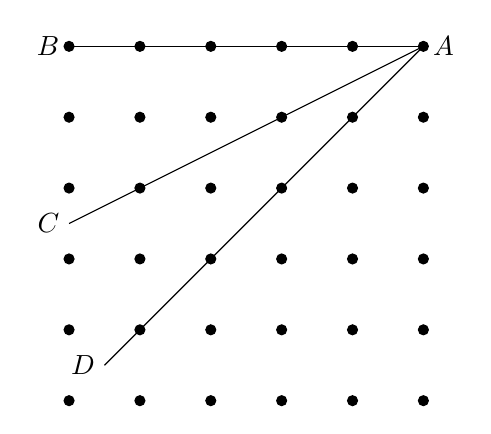
\begin{tikzpicture}[>=stealth,scale=0.9]
  \foreach \x in {0,1,2,...,5}
  \foreach \y in {0,1,2,...,5}
  {
  \draw [fill=black](\x,\y) circle (2pt);
  }
  
  \draw(0,5)node [left]{$B$}--(5,5)node [right]{$A$};
  \draw (5,5)--(0,3-.5)node [left]{$C$};
  \draw (5,5)--(.5,.5)node [left]{$D$};
\end{tikzpicture}
\end{document}